%\documentclass[xcolor=dvipsnames,12pt]{beamer}

% hide navigation symbols
\beamertemplatenavigationsymbolsempty

% add frame number
% TODO make it simplier
\makeatletter
\setbeamertemplate{footline}
{%
  \leavevmode%
  \hbox{%
  \begin{beamercolorbox}[wd=.92\paperwidth,ht=2.25ex,dp=1ex,center]{title in head/foot}%
  \end{beamercolorbox}%
  \begin{beamercolorbox}[wd=.08\paperwidth,ht=2.25ex,dp=1ex,leftskip=0cm plus1fill,rightskip=.015\paperwidth]{page number in head/foot}%
    \usebeamerfont{page number in head/foot}
    \insertframenumber{}
  \end{beamercolorbox}}%
  \vskip5pt%
}
\makeatother


% simple section page
\defbeamertemplate{section page}{simple}[1][]{
  \begin{centering}
    {\usebeamerfont{section name}\usebeamercolor[fg]{section name}#1}
    \vskip1em\par
    \begin{beamercolorbox}[sep=12pt,center]{part title}
      \usebeamerfont{section title}\insertsection\par
    \end{beamercolorbox}
  \end{centering}
}
\setbeamertemplate{section page}[simple]
\AtBeginSection{
  \frame[plain,c]{\sectionpage}
}

% mimic plain frame from metropolis theme
\newcommand{\plain}[2][]{%
  \begingroup
    \begin{frame}[plain,c]{#1}
      \begin{center}
        \usebeamercolor[fg]{frametitle}
        \bfseries\Large #2
      \end{center}
    \end{frame}
  \endgroup
}

% code colors
\colorlet{codeString}{Green}
\colorlet{codeKeyword}{RedOrange}
\colorlet{codeComment}{Gray}


% workaround for problem with white text if notes are enabled
% http://tex.stackexchange.com/questions/232168/normal-text-is-invisible-when-using-beamer-with-notes-and-xelatex
\def\pgfsysdriver{pgfsys-dvipdfm.def}

\documentclass[xcolor=dvipsnames]{beamer}

\usetheme{metropolis}
\setbeamercolor{normal text}{bg=white} % white background instead of black!2

% Fira Mono looks ugly, especially "0" & "&"
\setmonofont{Inconsolata}
% workaround for "Package polyglossia Error: The current roman font does not contain the Cyrillic script!"
\newfontfamily\cyrillicfonttt{Inconsolata}

% code colors from metropolis
\colorlet{codeString}{mLightGreen}
\colorlet{codeKeyword}{mLightBrown}
\colorlet{codeComment}{Gray}


\usepackage{ifxetex}

\ifxetex
  \usepackage{polyglossia}
  \setmainlanguage{russian}
  \setotherlanguage{english}

  % workaround for "Package polyglossia Error: The current roman font does not contain the Cyrillic script!"
  \newfontfamily\cyrillicfonttt{Fira Mono}
\else
  \usepackage[T2A]{fontenc}
  \usepackage[utf8]{inputenc}
  \usepackage[english,russian]{babel}

  % workaround for "Package hyperref Warning: Glyph not defined in PD1 encoding"
  \hypersetup{unicode=true}
\fi

\newcommand{\eng}[1]{%
  \ifxetex%
    {\textenglish{#1}}%
  \else%
    {\foreignlanguage{english}{#1}}%
  \fi%
}


\usepackage{pgfpages}
%\setbeameroption{show notes on second screen}

\usepackage{listings}
\lstset{
  basicstyle=\ttfamily,
  keywordstyle=\bfseries\color{codeKeyword},
  stringstyle=\color{codeString},
  commentstyle=\color{codeComment},
  literate={-}{-}1, % render dash as dash
  showstringspaces=false
}

\newcommand{\reduceBlockEqSpacing}{%
  \vspace*{-\baselineskip}\setlength\belowdisplayshortskip{0pt}%
}

% numbers formating: \num{123456}
\usepackage{numprint}
\newcommand{\num}[1]{\numprint{#1}}
  \npthousandsep{\,}
  \npthousandthpartsep{}
  \npdecimalsign{,}

\newcommand{\pcnum}[1]{\ensuremath{\mathtt{#1}}}
\newcommand{\bin}[1]{\pcnum{#1}_2}
\newcommand{\hex}[1]{\pcnum{#1}_{16}}

\newcommand{\code}[1]{\texttt{#1}}

\hypersetup{pdfauthor={Владимир Парфиненко}}
\title{Основы программирования}
\subtitle{Лекция № 2, 3 марта 2016 г.}
\date{}
\institute{
  \vspace{1em}
  \centering
  \parbox{0.9\textwidth}{
    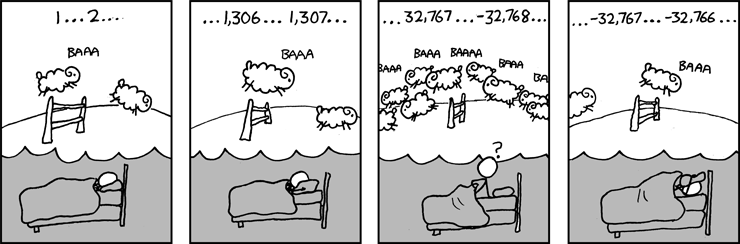
\includegraphics[width=\linewidth]{xkcd_cant_sleep}
    \par
    \raggedleft\tiny\url{http://xkcd.com/571}
  }
}


\begin{document}

\begin{frame}[plain]
  \titlepage
\end{frame}

\begin{frame}{Знакомство}

  Я~--- Владимир Парфиненко,

  \begin{itemize}
    \item бакалавр физики (ФФ), магистр математики (ММФ),
    \item профессиональный программист (Excelsior),
    \item регулярно чему-то учу (ФФ, АФТИ, ЛШ ФМШ).
  \end{itemize}

  Контакт:
  \href{mailto:vladimir.parfinenko@gmail.com}{vladimir.parfinenko@gmail.com}

\end{frame}

\section{Представление целых чисел}
\note{
  Порассуждать о том, как с помощью двух ламп можно представить числа от 0 до 3
}

\begin{frame}{Двоичная система счисления}

  Самый простой метод записи чисел, использующий только две цифры: 0 и 1.
  \note{компьютеру легко работать с такими числами\\}

  С помощью $n$ \emph{позиций} можно записать $2^n$ чисел.
  \note{Суффикс $x_{10}$ будем опускать\\}
  \begin{align*}
    \bin{000} &= 0, &\qquad \bin{100} &= 4, \\
    \bin{001} &= 1, &\qquad \bin{101} &= 5, \\
    \bin{010} &= 2, &\qquad \bin{110} &= 6, \\
    \bin{011} &= 3, &\qquad \bin{111} &= 7.
  \end{align*}
\end{frame}

\begin{frame}{Двоичная система счисления}

  Перевод из двоичной в десятичную:
  \[
    \bin{11001} = \mathbf{1} \cdot 2^4 + \mathbf{1} \cdot 2^3 +
                  \mathbf{0} \cdot 2^2 + \mathbf{0} \cdot 2^1 +
                  \mathbf{1} \cdot 2^0 = 16 + 8 + 1 = 25.
  \]
  Перевод из десятичной в двоичную:
  \note{сказать про обратный порядок\\}
  \begin{align*}
    25 &= 2 \cdot 12 + \mathbf{1}, \\
    12 &= 2 \cdot 6 + \mathbf{0}, \\
    6 &= 2 \cdot 3 + \mathbf{0}, \\
    3 &= 2 \cdot 1 + \mathbf{1}, \\
    1 &= 2 \cdot 0 + \mathbf{1}.
  \end{align*}

\end{frame}

\begin{frame}{Числа в памяти компьютера}

  1 \emph{байт} состоит из 8 \emph{бит} и может кодировать $2^8 = 256$
  различных чисел.
  \note{пояснить, что байт - минимальная ячейка памяти, которую компьютер может
  читать/писать\\}

  Например, число 337 кодируется минимум 2 байтами:
  \[
    \underbrace{\pcnum{00000001}}_{\text{биты } 15 \ldots 8}
    \underbrace{\pcnum{01010001}}_{\text{биты } 7 \ldots 0}
  \]

  Предельные значения:
  \begin{itemize}
    \item 8 бит: $0 \ldots \num{255}$,
    \item 16 бит: $0 \ldots \num{65535}$,
    \item 32 бита: $0 \ldots \num{4294967295}$,
    \item 64 бита: $0 \ldots \num{18446744073709551615}$.
  \end{itemize}
\end{frame}

\begin{frame}{Шестнадцатеричная система счисления}

  Цифры: $\pcnum{0}, \pcnum{1}, \pcnum{2}, \pcnum{3}, \pcnum{4}, \pcnum{5},
  \pcnum{6}, \pcnum{7}, \pcnum{8}, \pcnum{9}, \pcnum{A}, \pcnum{B}, \pcnum{C},
  \pcnum{D}, \pcnum{E}, \pcnum{F}$.

  Перевод в двоичную и обратно через тетрады (по 4 бита):
  \[
    \bin{101011100} = \pcnum{\{0001\}\{0101\}\{1100\}} = \hex{15C}.
  \]

  «Понятная» запись констант:
  \begin{itemize}
    \item 8 бит: диапазон чисел $\hex{0} \ldots \hex{FF}$,
    \item 32 бита: диапазон чисел $\hex{0} \ldots \hex{FFFFFFFF}$,
    \item $\texttt{0xDEADBEEF}, \texttt{0xCAFEBABE}, \texttt{0xCDCDCDCD},
      \ldots$
      \note{отладочная печать, Java-класс файл, неинициализированная память\\}
  \end{itemize}

\end{frame}

\begin{frame}{Знаковые числа}

  \note[item]{
  Отдельной памяти под знак нет, поэтому нужно упаковывать его в те же 8 (16,
  32, \ldots) бит.
  }

  \note[item]{
  Заметим, что компьютер выполняет сложение и вычитание по модулю,
  соответствующему размеру числа.
  }

  Рассмотрим сложение двух 8-битных чисел
  $\hex{FF} + \hex{01}$:
  \[
    \begin{array}{r}
    +
      \begin{array}{r}
        \pcnum{11111111} \\
        \pcnum{00000001} \\
      \end{array} \\
      \hline
      \begin{array}{r}
        \pcnum{1}\underbrace{\pcnum{00000000}}_{8 \text{ бит}}
      \end{array}
    \end{array}
  \]

  С точки зрения компьютера $(\hex{FF} + \hex{01}) \mod 2^8 = \hex{00}$.

  \visible<2->{
    \vspace{1em}
    То есть $X + 1 = 0$. Чему равно $X$?
  }

\end{frame}

\begin{frame}{Знаковые числа}

  Для представления отрицательных чисел используется \emph{двоичный
  дополнительный код}:
  \[ -X = 2^N - X, \text{где $N$~--- размер числа.}\]

  8-битные знаковые числа:
  \begin{align*}
    \bin{0000 0000} &= 0,    &\qquad \bin{1000 0000} &= -128, \\
    \bin{0000 0001} &= 1,    &\qquad \bin{1000 0001} &= -127, \\
                    &\ldots, &\qquad                 &\ldots, \\
    \bin{0111 1110} &= 126,  &\qquad \bin{1111 1110} &= -2,   \\
    \bin{0111 1111} &= 127,  &\qquad \bin{1111 1111} &= -1.
  \end{align*}

  \note{Сложение и вычитание не отличается от беззнаковых чисел.\par}
  \note{Умножение и деление~--- специфичное.\par}

\end{frame}

\begin{frame}{Переполнение}

  \begin{block}{Беззнаковые 8-битные:}
    \begin{itemize}
      \item $255 + 1 = \bin{1111 1111} + 1 = \bin{0000 0000} = 0$,
      \item $0 - 1 = \bin{0000 0000} - 1 = \bin{1111 1111} = 255$.
    \end{itemize}
  \end{block}

  \begin{block}{Знаковые 8-битные:}
    \begin{itemize}
      \item $127 + 1 = \bin{0111 1111} + 1 = \bin{1000 0000} = -128$,
      \item $-128 - 1 = \bin{1000 0000} - 1 = \bin{0111 1111} = 127$.
    \end{itemize}
  \end{block}

\end{frame}

\begin{frame}{\eng{Epic Fails}}

  \begin{itemize}
    \item 22 сентября 2009 г.~--- \eng{Twitter}: порядковый номер твитов
      переполнил 32-битное беззнаковое целое.

    \item 9 февраля 2013 г.~--- \eng{OpenStreetMap}: порядковый номер точек на
      карте переполнил 32-битное знаковое целое.

    \item 1 декабря 2014 г.~--- \eng{YouTube}: количество просмотров
      \href{https://www.youtube.com/watch?v=9bZkp7q19f0}{одного видео}
      переполнило 32-битное знаковое целое.
  \end{itemize}

  \note{В абсолютном большинстве случаев хватит 32-битных чисел.\par}

\end{frame}

\section{Целочисленные типы данных в \eng{C} и~операции над ними}

\begin{frame}{Беззнаковые целочисленные типы в \eng{C}}

  \begin{table}
    \begin{tabular}{ccc}
      \hline
      Тип              & Размер, бит & Максимум  \\
      \hline
      \code{unsigned char}      & 8  & $\num{255}$ \\
      \code{unsigned short}     & 16 & $\num{65535}$ \\
      \code{unsigned int}       & 32 & $\num{4294967295}$ \\
      \code{unsigned long long} & 64 & $\num{18.4e18}$ \\
      \hline
    \end{tabular}
  \end{table}

\end{frame}

\begin{frame}{Знаковые целочисленные типы в \eng{C}}

  \begin{table}
    \begin{tabular}{ccrl}
      \hline
      Тип              & Размер, бит & Минимум             & Максимум  \\
      \hline
      \code{signed char}        & 8  & $\num{-128}$        & $\num{127}$ \\
      \code{short}              & 16 & $\num{-32768}$      & $\num{32767}$ \\
      \code{int}                & 32 & $\num{-2147483648}$ & $\num{2147483647}$ \\
      \code{long long}          & 64 & $\num{-9.2e18}$     & $\num{9.2e18}$ \\
      \hline
    \end{tabular}
  \end{table}

\end{frame}

\begin{frame}{Арифметические операции}

  \begin{table}
    \begin{tabular}{cc}
      \hline
      Оператор      & Операция \\
      \hline
      \code{a + b}  & сложение \\
      \code{a - b}  & вычитание \\
      \code{a / b}  & деление нацело \\
      \code{a \% b} & остаток от деления \\
      \code{-a}     & отрицание \\
      \code{a++}    & инкремент \\
      \code{a-{}-}  & декремент \\
      \hline
    \end{tabular}
  \end{table}

\end{frame}

\begin{frame}[fragile]{Загадка: модуль числа неотрицательный?}

  \begin{block}{Вычисление модуля введенного числа:}
    \begin{lstlisting}[language=C]
    int x;
    printf("Enter number: ");
    scanf("%d", &x);
    if (x < 0) {
        x = -x;
    }
    printf("Absolute value = %d\n", x);
    \end{lstlisting}
  \end{block}

  \begin{block}{Исполнение:}
    \begin{onlyenv}<1>\begin{lstlisting}
    Enter number: -37
    Absolute value = 37
    \end{lstlisting}\end{onlyenv}
    \begin{onlyenv}<2>\begin{lstlisting}
    Enter number: -2147483648
    Absolute value = -2147483648
    \end{lstlisting}\end{onlyenv}
  \end{block}

\end{frame}

\begin{frame}{Битовые логические операции}

  \note{Целое число~--- это лишь набор битов.\\}

  \begin{block}{Бинарные:}
    \reduceBlockEqSpacing
    \[
      \text{\eng{AND} (\code{\&}):}\thickspace
      \begin{array}{r}
        \pcnum{0101} \\
        \pcnum{0011} \\
        \hline
        \pcnum{0001}
      \end{array}
      \qquad
      \text{\eng{OR} (\code{|}):}\thickspace
      \begin{array}{r}
        \pcnum{0101} \\
        \pcnum{0011} \\
        \hline
        \pcnum{0111}
      \end{array}
      \qquad
      \text{\eng{XOR} (\code{\textasciicircum}):}\thickspace
      \begin{array}{r}
        \pcnum{0101} \\
        \pcnum{0011} \\
        \hline
        \pcnum{0110}
      \end{array}
    \]
  \end{block}

  \begin{block}{Унарные:}
    \[
      \text{\eng{NOT} (\code{\textasciitilde}):}\thickspace
      \begin{array}{r}
        \pcnum{0101} \\
        \hline
        \pcnum{1010}
      \end{array}
    \]
  \end{block}

\end{frame}

\begin{frame}{Битовые сдвиги}

  Побитовый сдвиг беззнакового \code{x} на \code{n} бит...
  \begin{itemize}
    \item влево (\code{x <{}< n}) эквивалентен умножению на $2^n$,
    \item вправо (\code{x >{}> n}) эквивалентен делению на $2^n$.
  \end{itemize}
  \note{Сдвиг вправо для отрицательных чисел не специфицирован.\\}

  \begin{block}{Пример:}
    \reduceBlockEqSpacing
    \begin{equation*}
      \text{\code{<{}< 4}:}\thickspace
      \begin{array}{r}
        \pcnum{0101 \alert{1100 0011 0101}} \\
        \hline
        \pcnum{\alert{1100 0011 0101} 0000} \\
      \end{array}
      \qquad
      \text{\code{>{}> 4}:}\thickspace
      \begin{array}{r}
        \pcnum{\alert{0101 1100 0011} 0101} \\
        \hline
        \pcnum{0000 \alert{0101 1100 0011}} \\
      \end{array}
    \end{equation*}
  \end{block}

\end{frame}

\begin{frame}{Битовые операции на практике}

  \begin{block}{Чтение \code{i}-го бита из \code{x}:}
    \code{bit = (x >{}> i) \& 1;}
  \end{block}

  \begin{block}{Выставление \code{i}-го бита в \code{x}:}
    \code{x = x | (1 <{}< i);}
  \end{block}

  \begin{block}{Сброс \code{i}-го бита в \code{x}:}
    \code{x = x \& \textasciitilde(1 <{}< i);}
  \end{block}

\end{frame}

\section{Вещественные числа}

\begin{frame}{Представление вещественных чисел}

  Способы представления:
  \begin{itemize}
      \pause
    \item строка (\code{"\num{3.1415}"}),
      \note[item]{строки: произвольная точность}
      \pause
    \item рациональная дробь ($22/7 \approx \num{3.1429}$),
      \note[item]{дроби: абсолютная точность, используется в символьных
        вычислениях}
      \pause
    \item двоичная запись с фиксированной точкой\\
      ($\bin{\num{11.001001}} = 2^1 + 2^0 + 2^{-3} + 2^{-6} \approx
        \num{3.1406}$),
      \note[item]{фиксированная точка: предсказуемая точность, используется для
        финансов, быстрота (игровые приставки, кодирование звука/видео),
        ограниченный диапазон}
      \pause
    \item двоичная запись в плавающей точкой.
  \end{itemize}

\end{frame}

\begin{frame}{Числа с плавающей точкой}

  {\Large \[ x = m \cdot b^e, \] }
  где:
  \begin{itemize}
    \item $m$~--- \emph{мантисса} (значащая часть),
    \item $b$~--- \emph{основание степени} (обычно 2 или 10),
    \item $e$~--- \emph{экспонента} (порядок).
  \end{itemize}

\end{frame}

\begin{frame}{Стандарт IEEE 754}

  \begin{table}
    \begin{tabular}{r|cc}
                              & \eng{binary32}  & \eng{binary64} \\
      \hline
      тип в \eng{C}:          & \code{float}    & \code{double}  \\
      знак (бит):             & 1               & 1              \\
      экспонента (бит):       & 8               & 11             \\
      мантисса (бит):         & 23              & 52             \\
      точность (дес. знаки):  & 7               & 16             \\
      мин. абс. значение:     & \num{1.18e-38}  & \num{2.23e-308}\\
      макс. абс. значение:    & \num{3.40e38}   & \num{1.80e308} \\
    \end{tabular}
  \end{table}
  \note[item]{
    Точность binary32: $log_{10}(2^{23}+1) \approx \num{7.225}$,\\
    точность binary64 $log_{10}(2^{52}+1) \approx \num{15.955}$.
  }
  \note[item]{
    Мин. и макс. значения даны для нормализованных чисел.
  }

\end{frame}

\begin{frame}{Особенные числа}

  \newcommand{\NaN}{NaN}

  \begin{block}{Числа $\pm 0$, $\pm \infty$}
    \reduceBlockEqSpacing
    \begin{gather*}
      1 / (+0) = +\infty, \\
      1 / (-0) = -\infty, \\
      \log(0) = -\infty.
    \end{gather*}
  \end{block}

  \begin{block}<2->{Не-числа (\eng{NaN, Not a Number}):}
    \reduceBlockEqSpacing
    \begin{gather*}
      \NaN = \sqrt{-1}, 0 / 0, 0 \cdot \infty, \infty / \infty, \infty - \infty, \\
      \NaN = f(\NaN), \\
      \alert<3->{\NaN \neq \NaN}.
    \end{gather*}
  \end{block}

\end{frame}

\begin{frame}{Проблемы с точностью}

  \begin{itemize}
    \item Округление: $\tg(\pi) \neq 0, \tg(\pi/2) \neq \infty$.
    \item Накопление ошибок:
      $a \oplus (b \oplus c) \neq (a \oplus b) \oplus c$.
    \item Потеря точности:
      $a \ominus b$, при близких значениях $a$ и $b$.
      \note[item]{
        $(f(a)-f(b))/(a-b)$~--- в числителе значащими становятся младшие,
        неточные разряды}
    \item Сравнение чисел.
  \end{itemize}

\end{frame}

\begin{frame}[fragile]{Неправильное сравнение чисел}

  \begin{columns}[onlytextwidth,c]
    \begin{column}{0.6\textwidth}
      \begin{lstlisting}[language=C,escapechar=\!]
float x = 0.1f;
float y1 = x * x;
float y2 = 0.01f;

y1 == y2; !\visible<2->{\color{codeComment}// => 0}!
      \end{lstlisting}
    \end{column}

    \begin{column}<3->{0.4\textwidth}
      
\includegraphics[width=\linewidth]{meme_why}
    \end{column}

  \end{columns}

\end{frame}

\begin{frame}[fragile]{Причина неправильного сравнения чисел}

  \begin{lstlisting}[language=C,escapechar=\!]
float x = 0.1f; // 0.100000001490
float y1 = x * x;
// 0.010000000708 =
//    0 01111000 0100011110101110000101!\alert{1}!
float y2 = 0.01f;
// 0.009999999776 =
//    0 01111000 0100011110101110000101!\alert{0}!

y1 == y2; // => 0
  \end{lstlisting}

\end{frame}

\begin{frame}[fragile]{Правильное сравнение чисел}

  Идея:
  \begin{lstlisting}[language=C]
fabs(y1 - y2) < 0.00001f; // => 1
  \end{lstlisting}

  \pause

  Но нужно так же учесть:
  \begin{itemize}
    \item очень большие и очень маленькие числа,
    \item бесконечности,
    \item \ldots
  \end{itemize}

  Реализация: \href{%
    https://github.com/cypok/floats-comparison%
  }{%
    github.com/cypok/floats-comparison
  }

\end{frame}

\plain{Конец второй лекции}

\end{document}
